\chapter{Test phase \#1}\label{ch:test_1}

Afin de valider la phase 1 du développement du projet, un test impliquant le capteur choisi ainsi que la passerelle est effectué afin de s'assurer que les deux éléments sont capables de remplir les tâches qui leur sont attribuées pour le projet. Si le test est concluant, alors la solution matérielle choisie peut être validée pour la suite du développement. Dans le cas contraire le matériel doit être changé afin de pouvoir garantir une solution adéquate.

L'objectif est de vérifier le bon fonctionnement du capteur et de la passerelle dans les conditions finales d'utilisation, c'est-à-dire une réception adéquate des données envoyées par le capteur en extérieur et en mouvement. De plus ce test va également permettre de choisir la configuration initiale à utiliser pour la transmission des paquets LoRa, en particulier le facteur d'étalement ainsi que la puissance de transmission du signal de sortie à utiliser. On rappelle qu'un petit facteur d'étalement permettra un taux de transfert plus élevé sur une distance moindre, alors qu'un grand facteur permettra l'envoi de données à des distances accrues mais à un taux de transfert plus bas.

Pour pouvoir effectuer ce test, les éléments suivants ont été réalisés.

\begin{itemize}
\item Mise en place et assemblage du matériel du capteur et de la passerelle
\item Développement d'un programme de test pour le capteur
\item Installation et configuration du packet forwarder de la passerelle
\item Développement d'une partie du serveur d'application de la passerelle
\end{itemize}

Afin de pouvoir s'assurer de la bonne réception des données, le capteur, à intervalles réguliers, va envoyer un paquet de données à destination de la passerelle. Le format ainsi que le contenu du paquet envoyé par le capteur est décrit dans la figure~\ref{fig:test1_paquet}.

\begin{figure}[htb]
\centering 
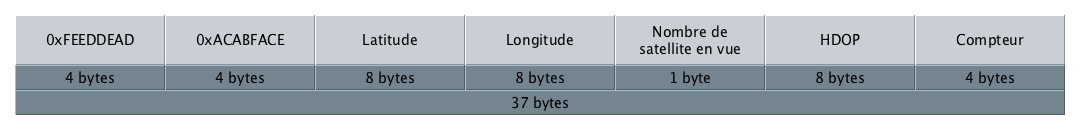
\includegraphics[width=1\columnwidth]{test1_packet_format.png} 
\caption{Format du paquet test1}
\label{fig:test1_paquet}
\end{figure}

Un programme de test, se basant sur le système de développement Arduino IDE proposant un framework pour les cartes Arduino, est réalisé. Son comportement est très simple, il se contente d'envoyer un paquet de données LoRa puis d'attendre un certain temps, au terme duquel le cycle recommence. Le paquet envoyé par le capteur commence par deux valeurs fixes suivies de la latitude/longitude du capteur au moment de l'envoi du paquet. Ces deux éléments sont suivis du HDOP, ou Horizontal Dilution of Precision, qui exprime le degré de précision de la position GPS. Pour terminer, la valeur du compteur est ajouté au paquet, ce qui permettra à la passerelle de détecter quand un paquet est perdu et ainsi garder des statistiques afin de pouvoir jauger la qualité de la transmission.

Du côté de la passerelle, le packet forwarder, logiciel repris depuis internet, est configuré et mis en œuvre. Il récupère les paquets LoRa reçus, les transforme en chaîne de text de type json et les transmet par le biais d'un paquet UDP. Une partie du serveur d'application est développée qui permet à la passerelle de récupérer les paquets LoRa émis par le packet forwarder au travers d'un socket et d'en analyser le contenu. A chaque paquet reçu, la passerelle s'assure que le paquet est en provenance du capteur en vérifiant la valeur des deux marqueurs de début, ensuite la valeur du compteur est vérifiée pour s'assurer que c'est bien celle attendue. Si ce n'est pas le cas, cela signifie qu'un ou plusieurs paquets ont été perdus dans l'intervalle. Cette partie du serveur d'application servira de base pour le développement final de l'application. 
Au moyen d'un shell implémenté dans le serveur de paquet, il est possible à tout moment de sauvegarder le contenu des paquets reçus jusqu'ici dans un fichier, cela permet ensuite d'en extraire les positions GPS afin de les afficher dans un logiciel comme Google Earth par exemple afin de permettre la visualisation de toutes les positions acquises durant le test.

Afin de pouvoir récupérer les logs relatifs aux tests et contrôler la réception des paquets, la passerelle est configurée afin de faire office de access point WiFi. Cela permet à l'ordinateur portable de se connecter à la passerelle au moyen de ssh et d'effectuer les opérations nécessaires.
Enfin, le capteur est alimenté par l'accumulateur polymer-ion et la passerelle, elle, est alimentée par l'USB de l'ordinateur portable.

Le code utilisé durant ce test correspond au tag de la version v0.1 sur git.

\begin{figure}[htb]
\centering 
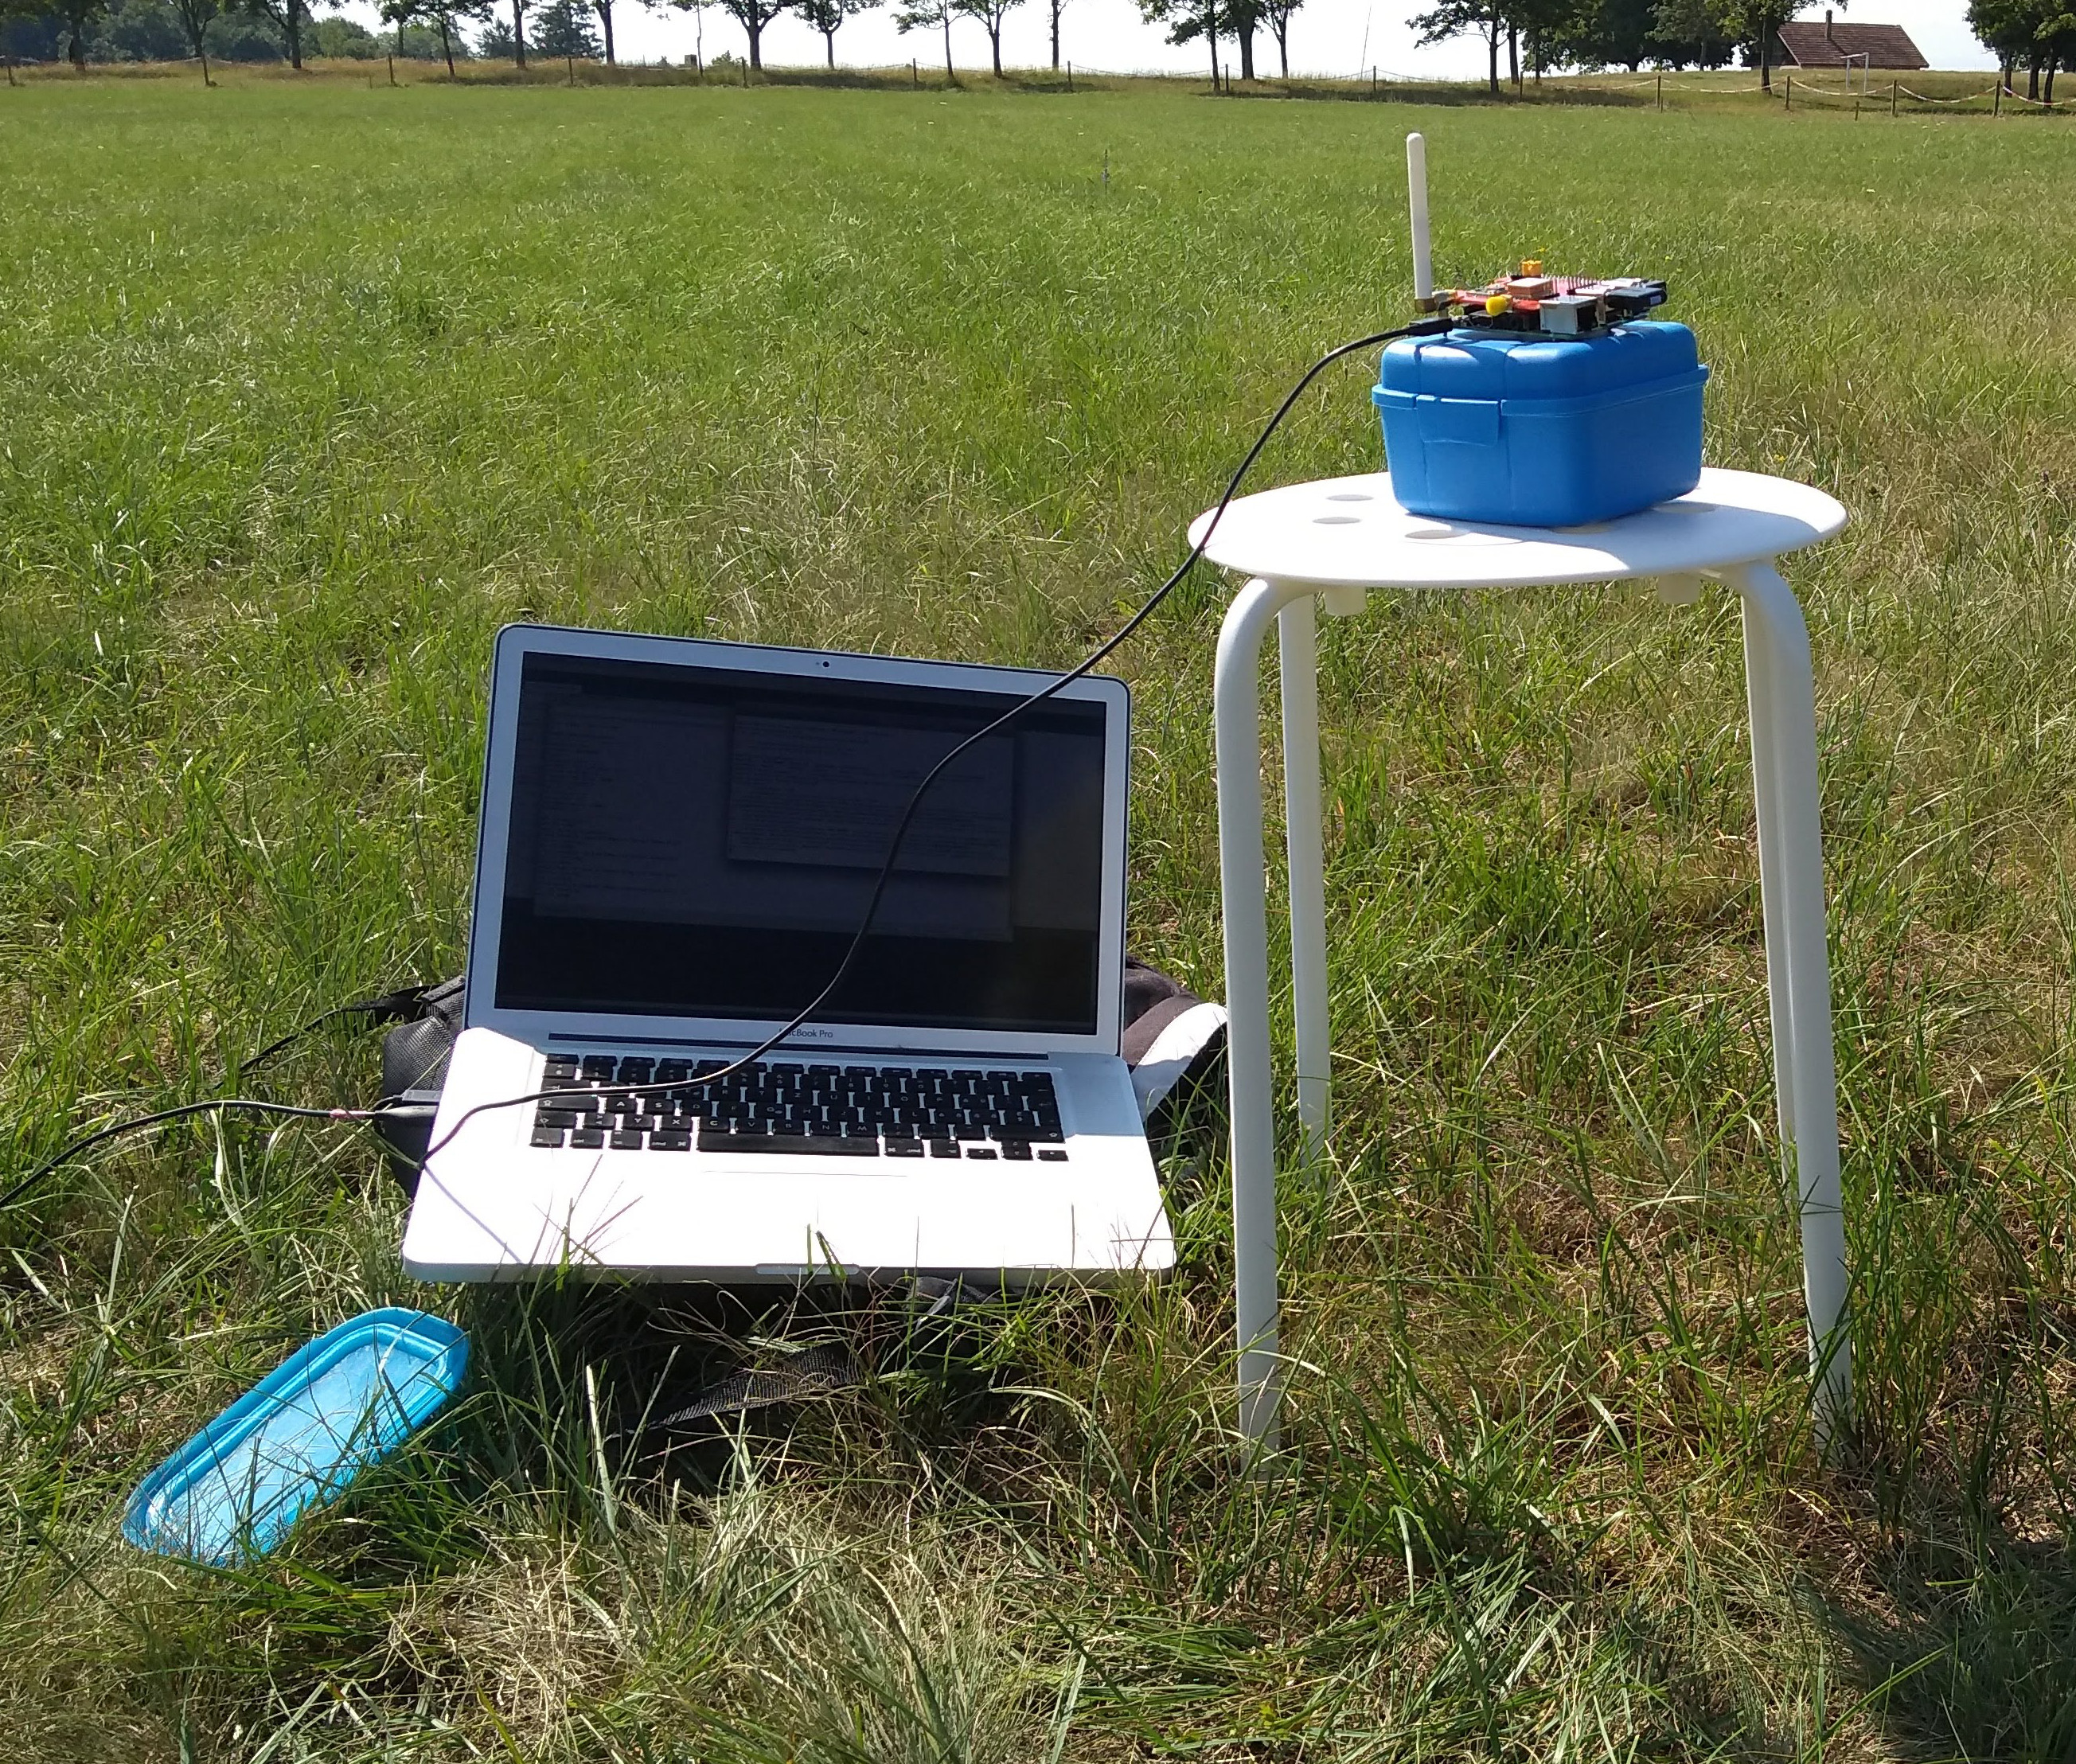
\includegraphics[width=0.7\columnwidth]{test_1_equip.jpg} 
\caption{Stituation pour le test \#1}
\label{fig:situation_test_1}
\end{figure}

\section{Scénarios}

Deux scénarios distincts sont réalisés en utilisant le système expliqué dans la section précédente. Ils seront effectués deux fois chacun, une fois avec la valeur d'étalement de spectre (spreading factor) avec la plus petite valeur et une fois avec la plus grande valeur, cela permettra de jauger quelle configuration sera nécessaire pour la version finale du capteur.

Le premier test est le test sur piste. Il consiste à prendre le capteur et ensuite de marcher le long du parcours d'une piste d'athlétisme. L'objectif de ce test est de voir si, dans des conditions proches de l'utilisation finale pour le projet, les données sont reçues correctement et de pouvoir également juger de la configuration finale que le système devra utiliser.

Le deuxième test est appelé test de distance, l'objectif et de pouvoir évaluer la distance maximum de fonctionnement jusqu'à laquelle les paquets sont bien reçus. Pour ce faire, le capteur sera déplacé sur une ligne droite jusqu'à un point fixé puis il sera retourné au point de départ.

\section{Résultats}

Les tests décrits dans cette section ont été réalisés à la place d'arme de Planeyse à Neuchâtel le 13 Juillet 2018. Cet endroit dispose de grandes surfaces planes et également d'une piste proposant des conditions très proche d'une piste d'athlétisme. C'est donc un endroit idéal réunissant les conditions nécessaires pour faire les tests.

Les  tables suivantes présentent les résultats des deux tests, sur piste et de distance. La colonne configuration spécifie les paramètres utilisés pour la communication LoRa, SF voulant dire spreading factor (facteur d'étalement) et PWR signifiant power (le niveau de puissance du signal en sortie).  Le facteur d'étalement peut être paramétré entre SF7 et SF12, le niveau de puissance quant à lui peut être configuré dans des valeurs entre -4.0 à +14.1 dBm.
Pour finir, les tables présentent également le nombre total de paquets reçus ainsi que le nombre de paquets perdus.

\subsection{Test sur piste}

\begin{table}[htb]
\caption[Résultats des tests phase 1 - Piste]{Résultats des tests phase 1 - Piste}
\label{tab:resultat_test_1_piste}
\centering
\begin{tabular}{lllllll}
\toprule
\multicolumn{4}{l}{ Tests Piste } & \multicolumn{3}{l}{ Planeyse 13.07.2018 } \\
\toprule
Nom & Configuration & HDOP Moy & Nb Sat Moy & Nb reçu & Nb perdu & \% perdu \\
\midrule
Test \#1 & SF7 - PWR -0.6 dBm & 0.97 & 8.74 & 46 & 3 & 6.1\% \\
Test \#2 & SF12 - PWR -0.6 dBm & 0.92 & 8.88 & 32 & 0 & 0  \\
\bottomrule 
\end{tabular}
\end{table}

Les figures~\ref{fig:test_piste_1} et~\ref{fig:test_piste_2} permettent de visualiser les positions GPS reçues dans chaque paquet LoRa. Lors du test, la passerelle était positionnée vers le centre de la piste, c'est de là que je suis parti avec le capteur, ce qui explique les premiers points qui ne se trouvent pas sur la piste.

\begin{figure}[htb]
\label{tab:resultat_tests_piste}
\centering
\begin{subfigure}[b]{1\textwidth}
   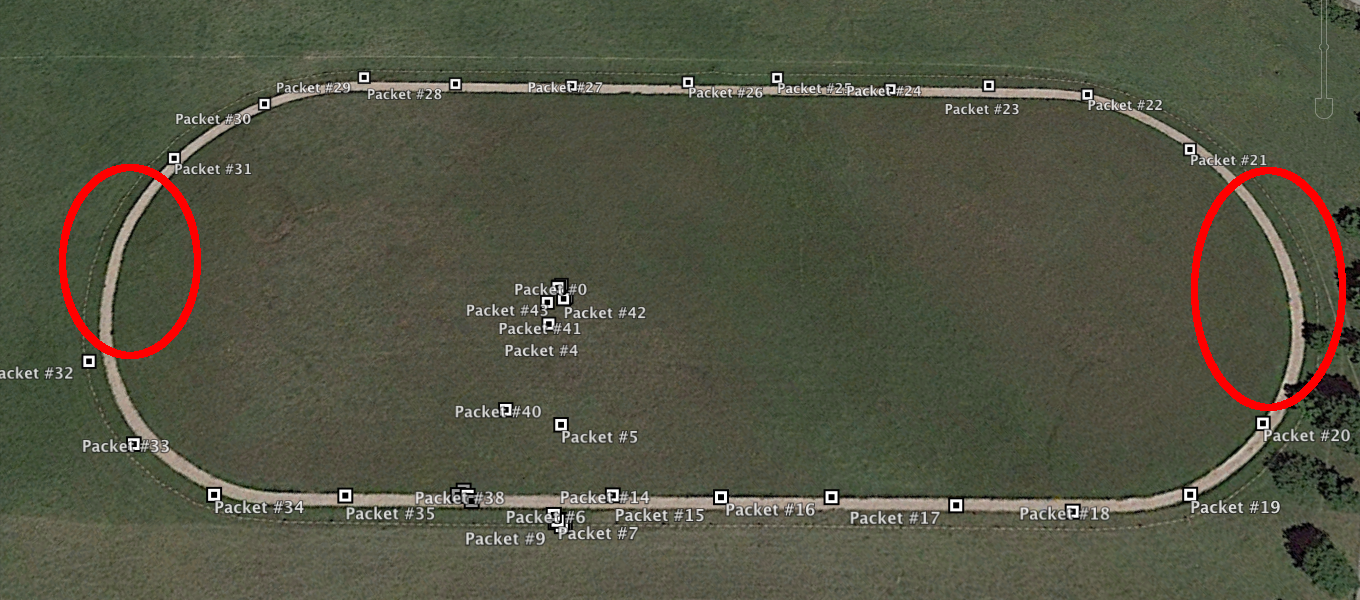
\includegraphics[width=1\linewidth]{test_planeyse_piste_1.png}
   \caption{Test \#1}
   \label{fig:test_piste_1}
\end{subfigure}

\begin{subfigure}[b]{1\textwidth}
   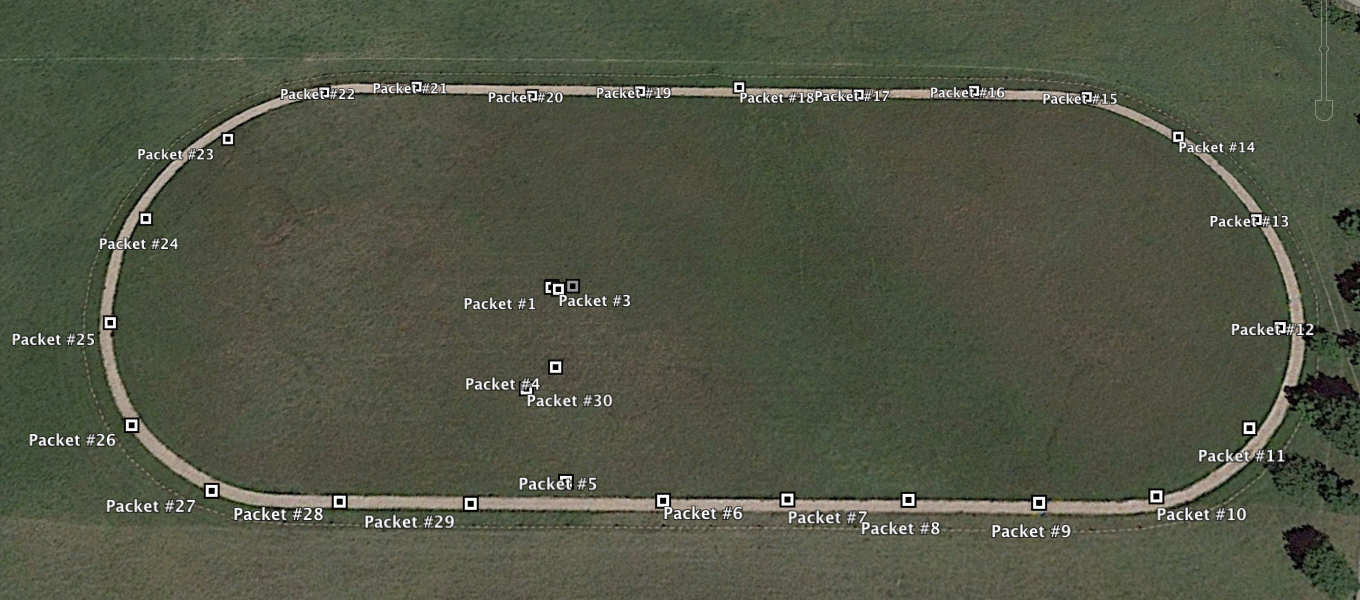
\includegraphics[width=1\linewidth]{test_planeyse_piste_2.png}
   \caption{Test \#2}
   \label{fig:test_piste_2}
\end{subfigure}
\caption[Positions GPS des tests piste]{Position GPS de chaque paquet reçu durant le test sur piste - Images capturées grâce au logiciel © Google Earth}
\end{figure}

On remarque que durant le test \#1 des paquets ont été perdus, dans les deux zones rouges, lorsque le capteur se trouvait aux extrémités de la piste. Lorsqu'on augmente la valeur du facteur d'étalement, dans le test \#2, on remarque que le problème n'apparait plus.

\subsection{Test de distance}

\begin{table}[htb]
\caption[Résultats des tests phase 1 - Distance]{Résultats des tests phase 1 - Distance}
\label{tab:resultat_test_1_distance}
\centering
\begin{tabular}{lllllll}
\toprule
\multicolumn{4}{l}{ Tests Distance } & \multicolumn{3}{l}{ Planeyse 13.07.2018 } \\
\toprule
Nom & Configuration & HDOP Moy & Nb Sat Moy & Nb reçu & Nb perdu & \% perdu \\
\midrule
Test \#3 & SF7 - PWR -0.6 dBm & 1.37 & 7.88 & 32 & 10 & 23.8\% \\
Test \#4 & SF12 - PWR -0.6 dBm & 0.93 & 9.32 & 37 & 1 & 2.6\%  \\
\bottomrule 
\end{tabular}
\end{table}

Les figures~\ref{fig:test_distance_1} et~\ref{fig:test_distance_2} permettent de visualiser les positions GPS reçues dans chaque paquet LoRa.

\begin{figure}[htb]
\centering
\begin{subfigure}{.5\textwidth}
  \centering
  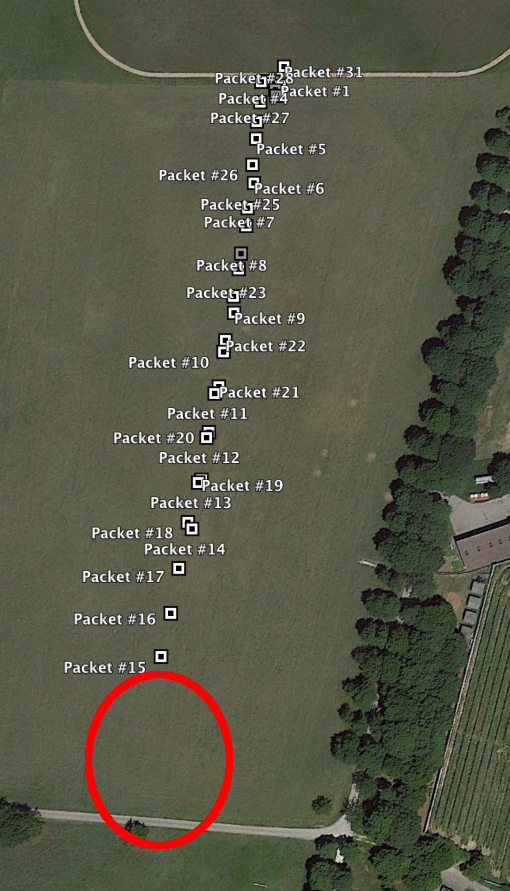
\includegraphics[width=.9\linewidth]{test_planeyse_distance_1.png}
  \caption{Test \#3}
  \label{fig:test_distance_1}
\end{subfigure}%
\begin{subfigure}{.5\textwidth}
  \centering
  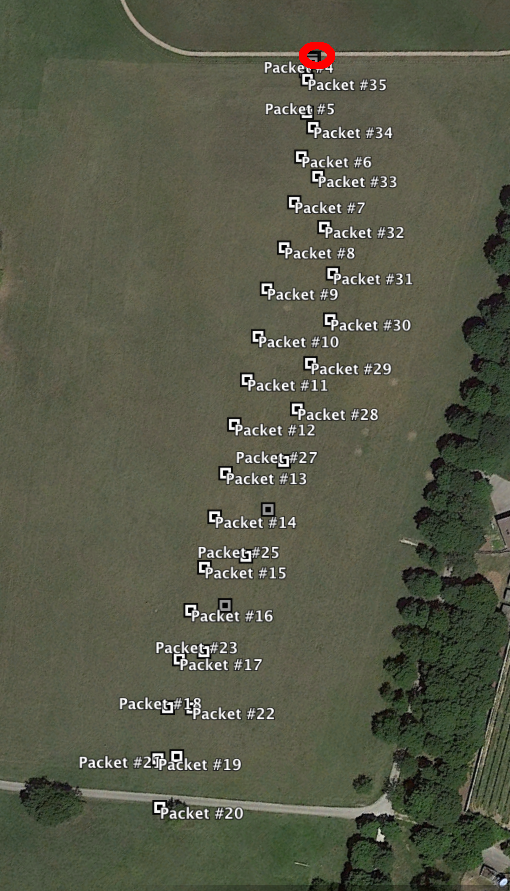
\includegraphics[width=.9\linewidth]{test_planeyse_distance_2.png}
  \caption{Test \#4}
  \label{fig:test_distance_2}
\end{subfigure}
\caption[Positions GPS des tests distance]{Position GPS de chaque paquet reçu durant le test de distance - Images capturées grâce au logiciel © Google Earth}
\label{fig:test_distance}
\end{figure}

Pendant les deux tests, quelques paquets ont été perdus dans les zones marquées en rouge. Cependant, si on analyse les résultats plus en détail, on remarque que durant le test \#4, un seul paquet a été perdu et ce au moment où le capteur était très proche de la passerelle, on peut donc négliger cette perte qui est probablement due à un masquage de l'antenne de la passerelle. 
Lors du test \#3 par contre, la distance limite qu'il est possible d'atteindre avec la configuration SF7 et puissance à -0.6 dBm a été atteinte après environ 200m de distance entre le capteur et la passerelle.

\section{Conclusions}

Au terme du test phase \#1 on peut conclure que:

\begin{itemize}
\item La précision des positions GPS fournis par le module GPS est suffisante pour l'application visée
\item Le fait que le capteur soit en mouvement ne pose pas de problème au niveau de la couche radio LoRa ou de la qualité des positions GPS fournies
\item L'alimentation du capteur par l'accumulateur et la passerelle par l'USB fonctionne correctement
\item La configuration de la couche radio devra être adaptée, le facteur d'étalement SF7 et puissance à -0.6 dBm n'étant pas suffisant pour un taux de réception de paquet satisfaisant
\end{itemize}

Grâce à ses éléments, on peut conclure que le matériel choisi est adéquat, la phase \#1 du développement du projet est donc validée, ce qui permet donc de passer à la phase \#2. Dans cette phase du projet, la base de données, l'application du capteur et une ébauche de l'application mobile seront développées, ce qui permettra de pouvoir tester la chaîne de communication complète du système.





